\chapter{Introdução}
\label{cap:introducao}

A extração de petróleo em ambiente marítimo constitui uma das atividades de engenharia de maior complexidade operacional e volume de investimento de capital \cite{CHAKRABARTI20051}, mantendo papel estratégico na segurança e no suprimento da matriz energética mundial \cite{iea2025world}. Os esforços em Pesquisa e Desenvolvimento (P\&D) envolvidos nessas operações são cruciais para superar os desafios tecnológicos, especialmente em águas profundas \cite{Morais_2011}. Esse processo, que se inicia com campanhas exploratórias e culmina na produção efetiva, é realizado a partir de estruturas especializadas, as plataformas de petróleo, e exige um rigoroso licenciamento ambiental em todas as suas fases, dada a necessidade de compreender e mitigar os impactos ambientais gerados pela atividade \cite{Martins_2015}.

De acordo com \cite{MME_2023}, a etapa de desenvolvimento do campo de petróleo e gás natural envolve a perfuração de poços e a instalação de um complexo sistema submarino, havendo diversas técnicas para a construção e montagem de uma plataforma, sendo um dos fatores determinantes a profundidade do campo de petróleo e gás. Em profundidades de até 400 metros, o tipo de plataforma é considerada de águas rasas, e sua estrutura pode ficar sobre torres de concreto e aço, capazes de aguentar todas as intempéries do tempo e mar revolto. Já no caso de uma maior profundidade, fazendo com que a plataforma esteja parcialmente submersa, as plataformas são do tipo semissubmersíveis, tendo uma maior estabilidade, visto que esse são instalados pontos de ancoragem para evitar que as instalações fiquem à deriva no oceano. Por fim, existe a chamada \gls{FPSO}, que são navios com capacidade de processar, armazenar e transferir petróleo e gás natural a outros navios.

Com a perfuração do poço, feita por meio do uso de uma broca com dente de aço, é necessária a instalação do equipamento de segurança chamado \gls{BOP}, que pode ser visto na imagem \ref{fig:bop}. Esse dispositivo consiste em um sistema hidráulico ou eletro-hidráulico fundamental para vedar o poço e prevenir acidentes de vazamento sob alta pressão. Para conectar o \gls{BOP} na cabeça do poço à unidade de perfuração na superfície, utiliza-se do \textit{drilling riser}, que é uma coluna tubular essencial que atua como um conduto de retorno dos fluidos de perfuração e guia para as ferramentas. Há também a chamada Árvore de Natal Molhada, que pode ser vista na Figura \ref{fig:arvore_natal_molhada}, um conjunto de válvulas que gerencia o fluxo de produção. A operação de instalação desses equipamentos críticos, como o lançamento e descida dos \textit{risers} e o assentamento do \gls{BOP} no solo marítimo, representa um dos maiores desafios logísticos e de segurança em sistemas de perfuração marítima \cite{Tsukada_2007}. O produto final (petróleo e gás) é escoado por dutos ou navios petroleiros.

\begin{figure}
    \centering
    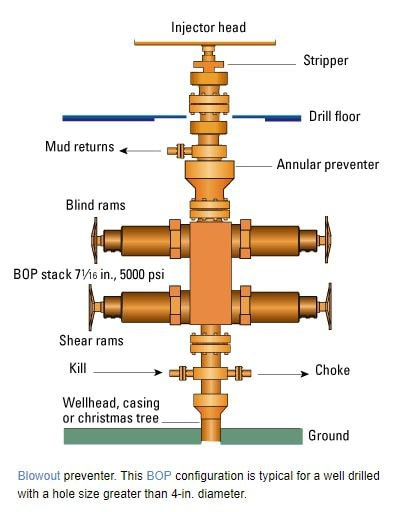
\includegraphics[width=0.5\linewidth]{figuras/BOP.jpg}
    \captionsetup{justification=centering}
    \caption{\gls{BOP}}
    \label{fig:bop}
\end{figure}

\begin{figure}
    \centering
    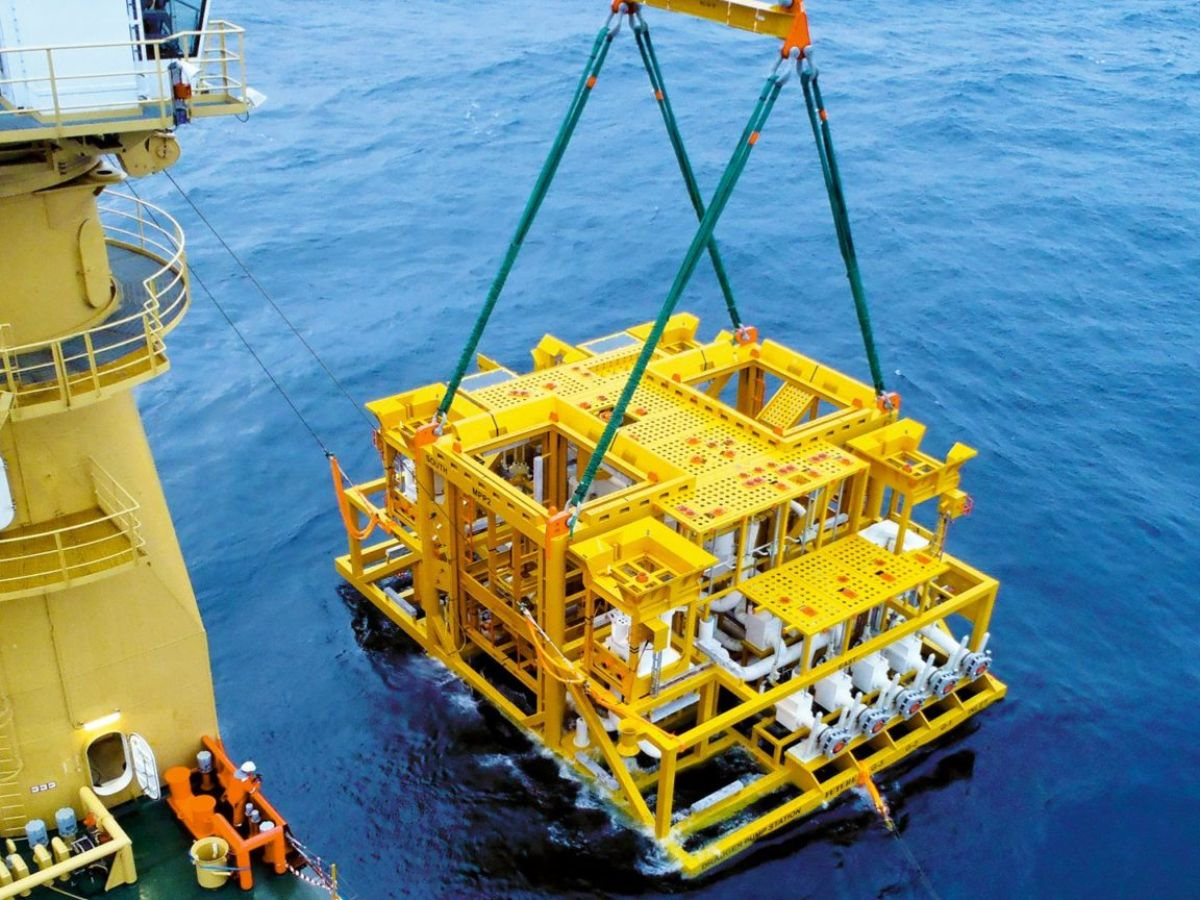
\includegraphics[width=0.5\linewidth]{figuras/arvore_natal_molhada.jpg}
    \captionsetup{justification=centering}
    \caption{Árvore de Natal Molhada}
    \label{fig:bop}
\end{figure}

Quanto à simulação numérica de reservatórios, este é um método amplamente reconhecido e eficaz para a exploração de questões complexas e o estudo do comportamento de fluxo em condições reais de reservatório \cite{Sikanyika_2023_Numerical}. Devido ao alto custo e aos desafios operacionais, especialmente em campos \textit{offshore} e reservatórios de baixa permeabilidade, a indústria busca sempre melhorar a produção, com menos poços, tornando a precisão e a eficiência da modelagem críticas \cite{Wu_2025_OptimizationWellPatterns}.

A modelagem de reservatórios é governada por equações diferenciais parciais que descrevem o fluxo de fluidos (óleo, gás, água) em meios porosos, como as equações do modelo \textit{Black-Oil} \cite{Sikanyika_2023_Numerical}. Além da complexidade do reservatório, a simulação detalhada de componentes do poço também exige a solução de equações de alta complexidade. Por exemplo, a otimização de dispositivos de controle de fluxo requer a aplicação de \gls{CFD} para resolver as equações de continuidade e de momento para escoamento turbulento, muitas vezes empregando modelos como o $k-\epsilon$ \cite{Gao_2023_DesignNumerical}.

O tempo de processamento demandado pelos modelos de alta fidelidade — que pode alcançar horas ou dias para a simulação de um único cenário em campos complexos — configura uma importante oportunidade de ganho de eficiência computacional. A redução desse tempo de resposta potencializa a execução e amplia o alcance de tarefas de gerenciamento e otimização que dependem de múltiplas avaliações sucessivas, tais como:

\begin{itemize}

\item \textbf{\gls{UQ}}: A avaliação robusta da incerteza dos parâmetros do reservatório (porosidade, permeabilidade, etc.) exige a execução de milhares de simulações (e.g., Monte Carlo) \cite{Wu_2025_OptimizationWellPatterns}.

\item \textbf{Otimização de Produção e Otimização Econômica}: A busca pelo posicionamento ideal de poços ou pela maximização do Valor Presente Líquido (VPL) envolve a iteração contínua sobre diversos parâmetros (espaçamento, fraturamento, padrões de injeção), sendo impulsionada pelo uso de modelos ágeis para avaliar cada tentativa \cite{Wu_2025_OptimizationWellPatterns}.

\item \textbf{Estudo de Cenários}: A comparação entre diferentes estratégias, como poços horizontais versus verticais com injeção de água, pode ser substancialmente expandida ao se viabilizar um maior número de iterações em busca de maior eficiência de recuperação \cite{Sikanyika_2023_Numerical}.

\end{itemize}

Diante desse panorama, a literatura recente tem explorado amplamente a interseção entre computação de alto desempenho e técnicas de \gls{IA} para contornar tais restrições temporais. Conforme destacado por \citeonline{portella2022tunaoil}, a simulação de fluxo em reservatórios e a imagiologia sísmica constituem as cargas de trabalho mais intensivas em supercomputadores no setor de óleo e gás, motivando o desenvolvimento de estratégias inteligentes que acelerem o tempo de resposta sem comprometer o rigor dos resultados. Enquanto abordagens como o \textit{TunaOil} atuam na sintonização de parâmetros internos do próprio simulador numérico para otimizar o tempo de CPU, uma vertente complementar e altamente promissora consiste no emprego de modelos substitutos. Por meio dessa abordagem, algoritmos de \gls{ML} são treinados a partir de históricos e execuções prévias para emular o comportamento das variáveis de interesse com baixo custo computacional, permitindo que rotinas complexas de otimização matemática explorem amplamente o espaço de busca e acelerem a tomada de decisão estratégica no desenvolvimento do campo.

A estrutura deste trabalho está organizada em capítulos que detalham o problema abordado, o embasamento teórico, os métodos utilizados nos experimentos e resultados obtidos. A organização segue a seguinte ordem:

\begin{itemize}
    \item \textbf{Capítulo \ref{cap:problema}:} Define formalmente o problema de previsão de vazão, estabelecendo as modelagens matemáticas para as abordagens linear e não linear, além de descrever as métricas estatísticas utilizadas para a otimização dos modelos.
    \item \textbf{Capítulo \ref{cap:fundamentacao-teorica}:} Reúne a fundamentação teórica necessária para a compreensão dos conceitos de extração de petróleo \textit{offshore}, modelagem \textit{surrogate} e os princípios matemáticos dos algoritmos de Aprendizado de Máquina selecionados.
    \item \textbf{Capítulo \ref{cap:proposta-e-metodologia}:} Detalha o fluxo metodológico, abrangendo a extração de dados no sistema de \gls{CDP}, o processo rigoroso de limpeza de dados \icaroC{(\textit{Data Cleansing})}, a engenharia de atributos e a configuração dos experimentos computacionais.
    \item \textbf{Capítulo \ref{cap:experimentos}:} Expõe os resultados alcançados, apresentando a comparação de desempenho entre os modelos lineares, de conjunto e redes neurais, baseando-se nas métricas de erro estatístico e custo computacional.
    \item \textbf{Capítulo \ref{cap:conclusao}:} Sintetiza as principais conclusões obtidas, discute as limitações da pesquisa e propõe sugestões de trabalhos futuros para o aprimoramento da modelagem preditiva em sistemas de produção.
\end{itemize}